\section{Door task}
	\label{sub:door}

\subsection{Outline of door task}
%
In DRC Finals, the door task has special importance, because without passing it, a robot could not approach five rest tasks (valve, wall, surprise, debris or terrain, and stairs).
   
In general, we can separate door passing task into the following phases.
%
\begin{enumerate}
\item Walk to the front of the door 
\item Grasp the door knob
\item Turn the knob and open the door
\item Walk through the door
\end{enumerate}
%

%In the DRC Finals, it was announced that the door will be 
%
%\begin{itemize}
%\item push open style,
%\item with lever type door knob, and
%\item without door closer.
%\end{itemize}

At the end of the second phase, a robot get a pose standing with a hand grasping 
the door lever. Let us call this the {\it open-door pose} as illustrated in \figurename~\ref{fig:door_approaching_config}.
In our approach, we specify a specific standing point and a wrist positioning with respect to 
the door lever as shown in the figure.
By this way, the rest phases 3) and 4) start from the same configuration, thus we can 
use a pre-programmed sequence for the door operation and door passing.
Even we face variations of door geometry, it can be handled by minimum modification by this way.

\begin{figure}[t]
  \centering
  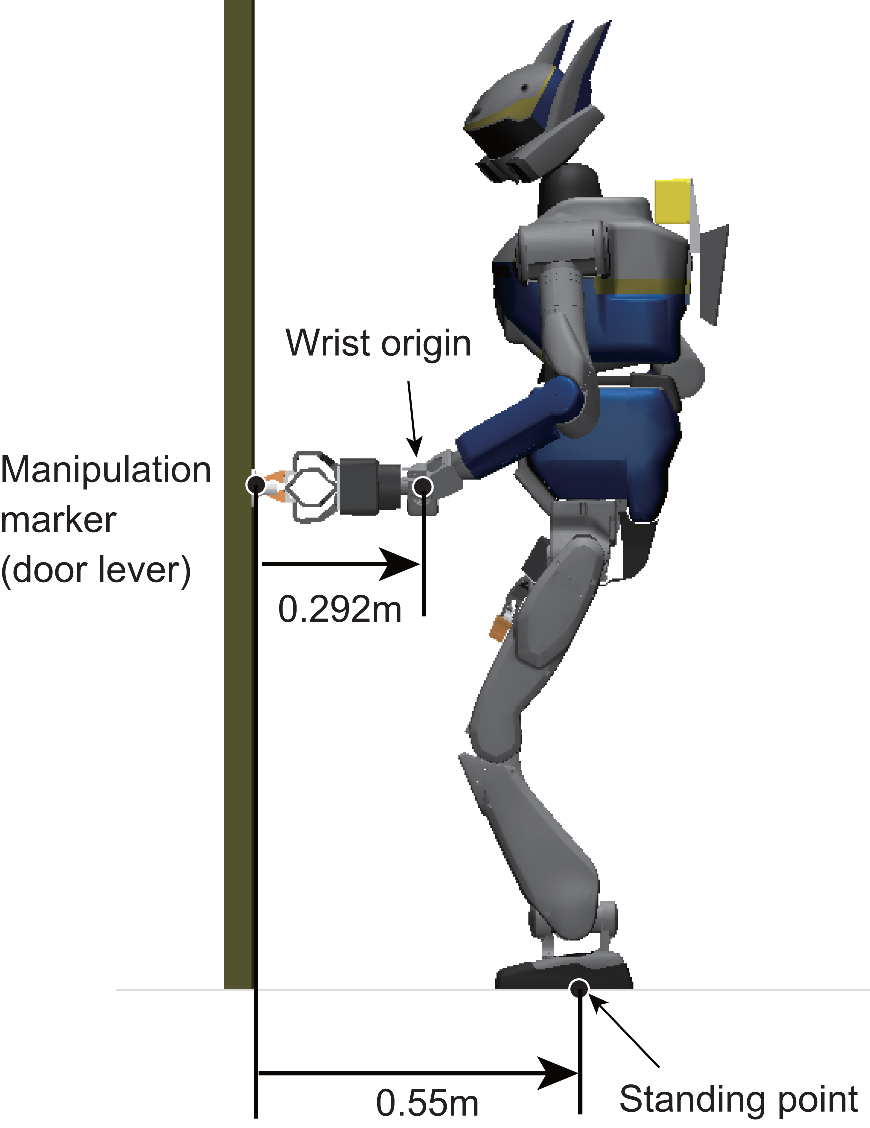
\includegraphics[width = 6cm]{img/door_approaching_config}
  \caption{Open-door pose}
  \label{fig:door_approaching_config}
\end{figure}

%From Step1 to Step2, we control our robot to realize the door approaching pose.
%To realize a reliable door passing, we pre-determined
%a robot pose grasping the door knob.
%Let us call it as {\it door approaching pose} which specifies the
%wrist point and the standing point with respect to the door lever

%The door knob operation (Step3) and the door passing through (Step4) always start
%from this fixed configuration. This means we can use a programmed sequence or its minimum
%modification at the door task.  

In the following subsections, we explains phase 1) and 2), the way of robot control to get the open-door pose
by the sensor information and teleoperation. The phase 3) and 4) can be easily implemented. 
Especially in the DRC Finals, once the door was opened enough, it opened by gravity
and remained opening, since the door hinge was inclined 2.6 degrees from vertical.
This helped robots walk though without worrying collision with the opened door, which eventually hit the
robot by wind in usual case. 

\subsection{Walk to the front of the door}
%
To navigate a robot to the position as specified in \figurename~\ref{fig:door_approaching_config}, we use
point cloud data measured by LRF. 
We took two step manual operations to identify the door orientation and the position of the door lever 
as illustrated in Fig.\ref{fig:door_manip_markers}.

First, an operator specifies a point on the point on the left edge of the door panel (\figurename~\ref{fig:door_manip_markers}(a) `x' mark pointed by arrow). By applying the least square method to the point cloud exist on the right of the specified point, we can calculate the orientation of the door panel.
The result is shown by the {\it door marker}, a gray rectangle in \figurename~\ref{fig:door_manip_markers}(b).
It covers a part of the door panel and we can interactively manipulate it on the 
point cloud GUI. By adjusting the door marker, we can mask the points for the door panel and extract the points for the door lever as shown in \figurename~\ref{fig:door_manip_markers}(c).
%Since the door lever is relatively small with respect to the point cloud resolution,
%it contains only 10 to 20 points which makes conventional model fitting very difficult.
%Thanks to the robustness of the human perception, 
By this way, we can confidently mark the rotation center of the lever (pointed by arrow).
Figure \ref{fig:door_manip_markers}(d) show the manipulation marker for the door lever placed on the point cloud. Its position and orientation is used to navigate the robot to the desired point for door opening.

\begin{figure}[t]
  \centering
  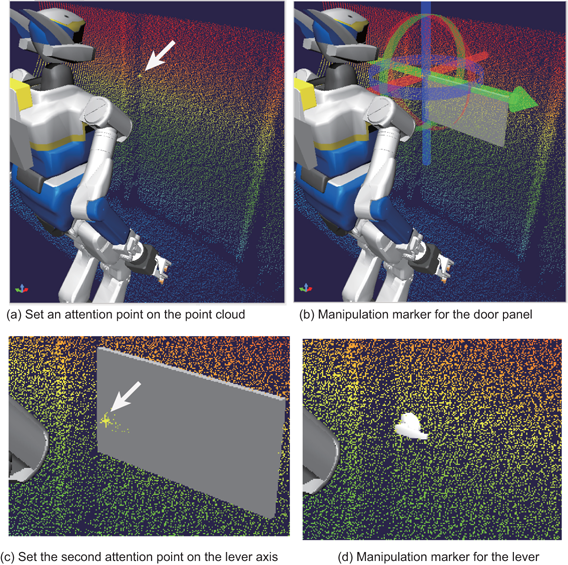
\includegraphics[width = 7.5cm]{img/door_manipulation_markers}
  \caption{Detection of the door lever in the control window}
  \label{fig:door_manip_markers}
\end{figure}
		

\subsection{Grasp the door knob}
%
Now the robot is standing on the good place to grasp the door knob.
%By the method of previous subsection, we can expect our robot is standing in front of the door aligned to its surface normal with desired distance.
Instead of grasping the door knob directry, we move the robot hand to an {\it approach point},
which is placed at a certain distance (0.13m) from the knob. 
Because, the hand position may not be accurate enough due to the LRF measurement noise, calibration error,
and the slip of walking.

Figure \ref{fig:door_lever_grasp}(a) show the robot at the open-door pose whose hand is at the approach point (right window) in Choreonoid simulator. The left window shows the simulated view of the left hand camera. Both images show that the left hand is appropriate to grasp the door knob. Note that in real robot control, only the camera view is available. 

 An operator can manually adjust the hand position by the GUI buttons of 
{\it Left},{\it Right},{\it Down}, and {\it Up} as seen in the left window bottom. In this case, an operator
can adjust the hand position by hitting {\it Right} button several times.
Figure \ref{fig:door_lever_grasp}(b) shows the adjusted hand position to grasp the lever.

Figure \ref{fig:door_lever_grasp}(c) show the final state getting the good grasp of the door lever. From this moment, the point cloud based manipulation marker is no longer used. For example, the center of the knob rotation is determined using the hand position calculated from the internal sensors (joint encoders and posture sensors). 
%By hitting the button 'OK', the robot move the left hand forward until it contacts the door surface (we specified a sleshold of 5N to detect the contact).  The hand is in contact with appropriate position to grasp the door lever in \figurename~\ref{fig:door_lever_grasp}(c).
%
\begin{figure}[t]
  \centering
  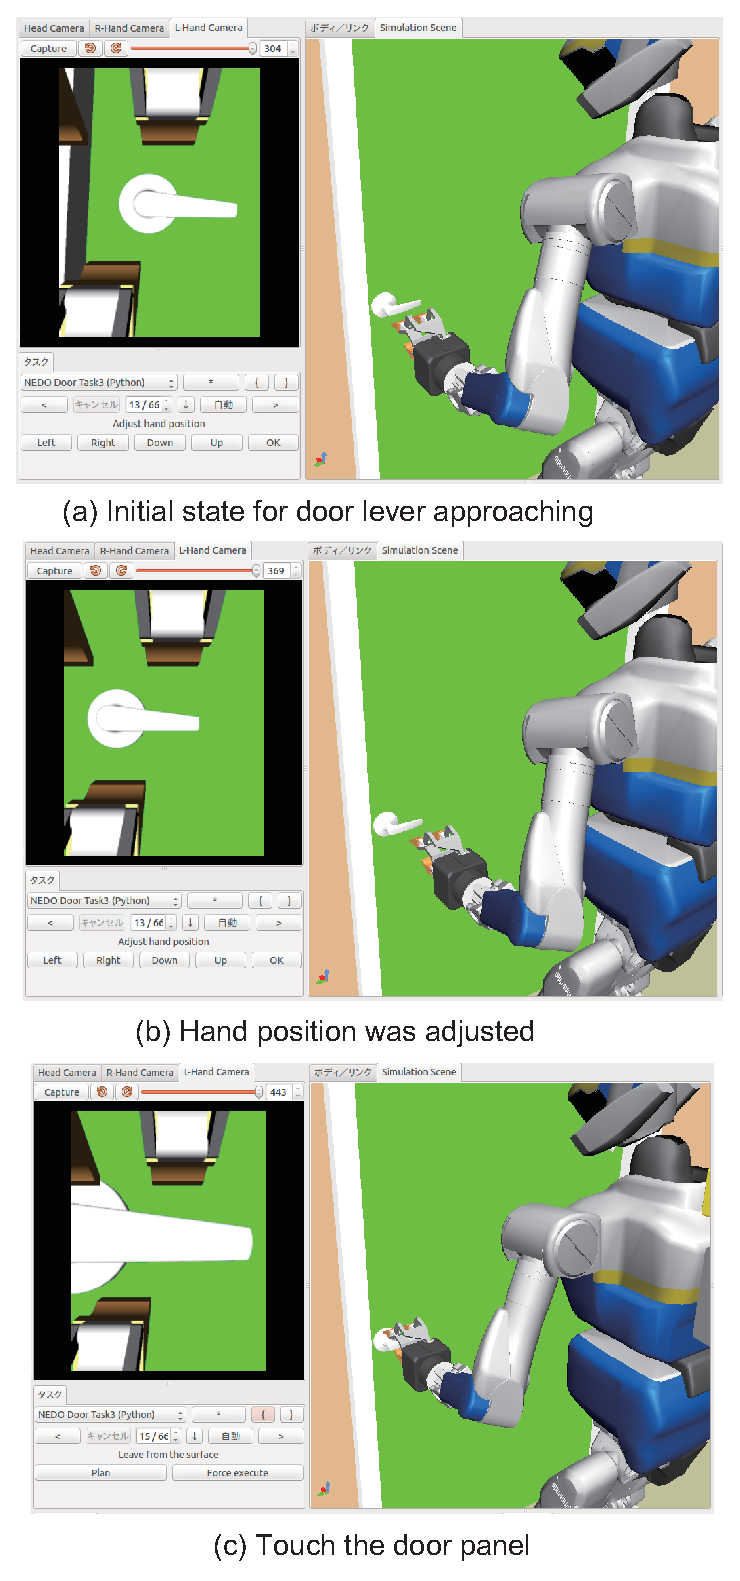
\includegraphics[width = 7.5cm]{img/approach_door_lever}
  \caption{Approach for door lever grasping}
  \label{fig:door_lever_grasp}
\end{figure}

%\begin{figure}[t]
%  \centering
%  \includegraphics[width = 7.5cm]{img/open_the_door}
%  \caption{Door opening}
%  \label{fig:door_opening}
%\end{figure}

\subsection{Results at DRC Finals}
%
In the DRC Finals 2015, HRP-2Kai cleared the door task in the rehasal on June 4 and in
the challenge on June 6. Figure \ref{fig:drc_door_aist_day2} shows the robot (a) scanned LRF 
to obtain point cloud, (b) walked to the point of the opendoor pose, (c) grasp the door lever, and (d)
 opend the door successfully. The robot spent 5 minute 21 seconds from the LRF scanning to get the 
robot fully passed the door.
%
\begin{figure}[t]
  \centering
  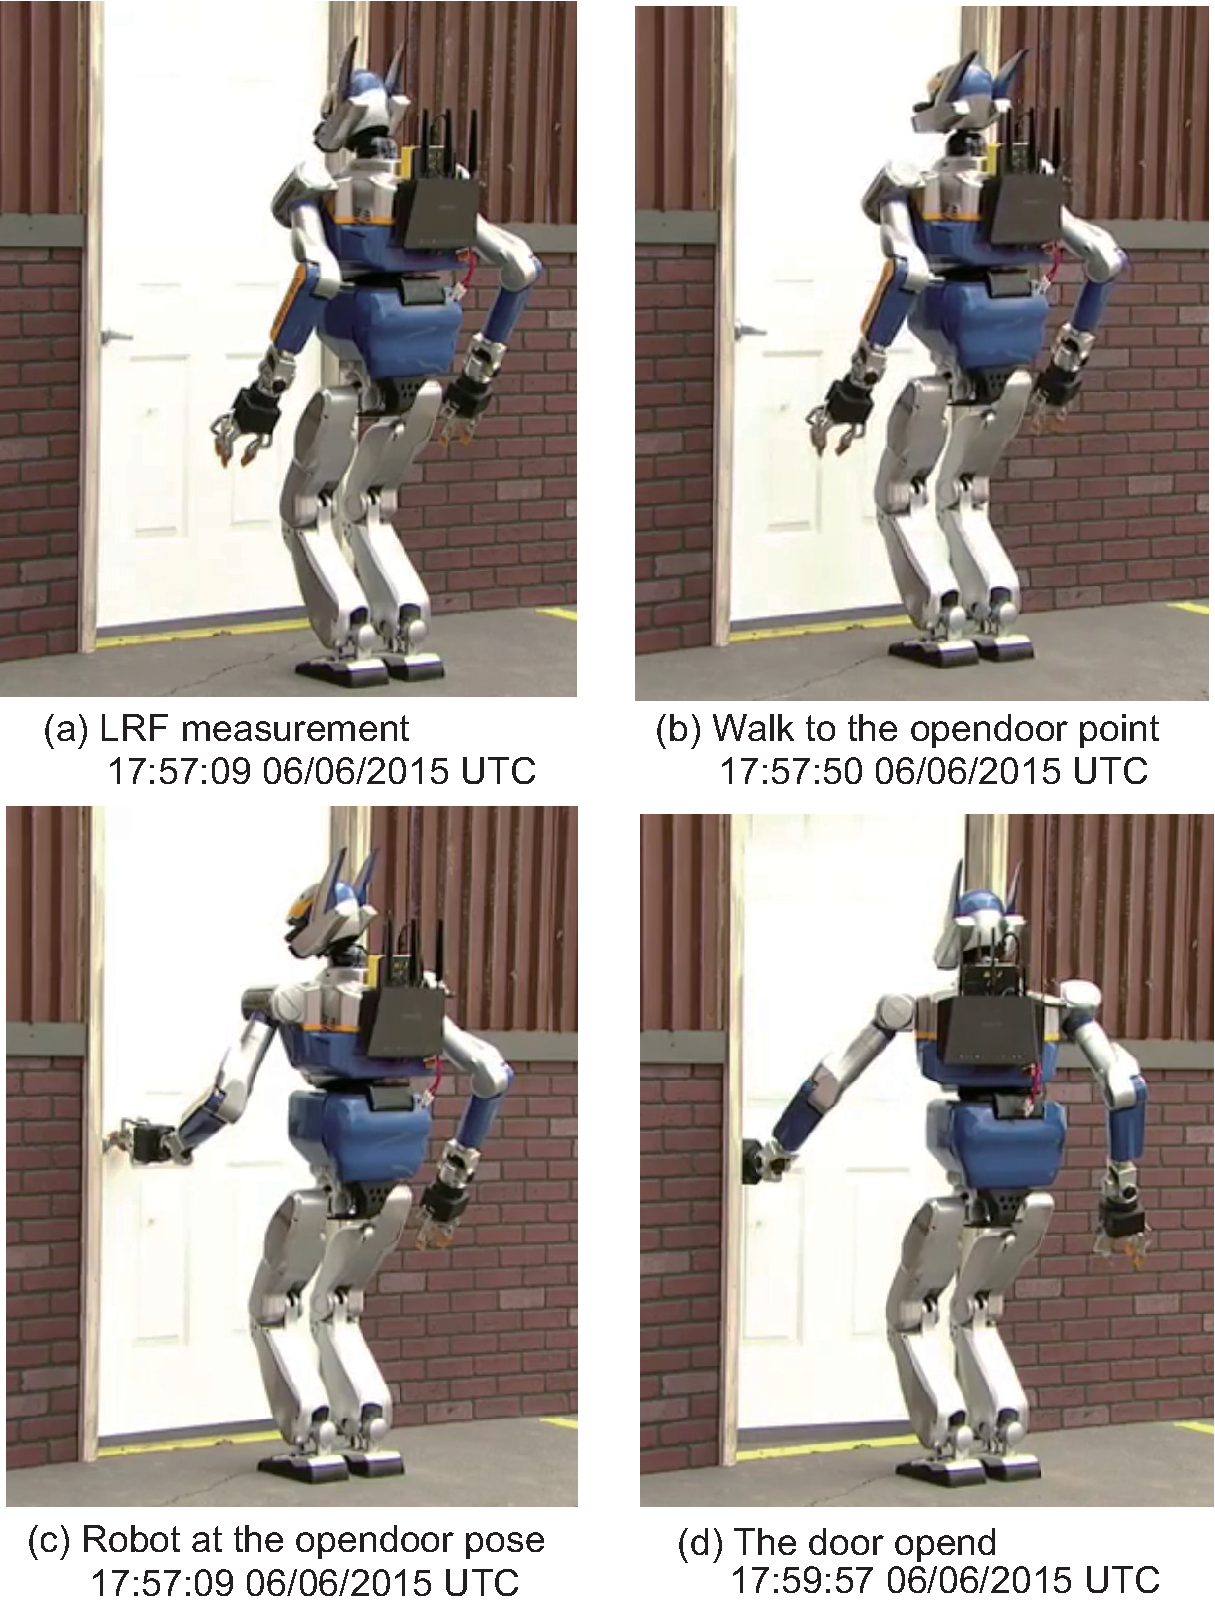
\includegraphics[width = 7.5cm]{img/drc_door_aist_day2}
  \caption{Door task at DRC Finals on June 6}
  \label{fig:drc_door_aist_day2}
\end{figure}

In the challenge on June 5, HRP-2Kai failed the door lever operation and tried to
grasp again by manual teleoperation. During this operation, we had a low level control system crash, 
and the robot had fell (\figurename~\ref{fig:drc_door_aist_day1}).
Since we had the computer stopped as well as the hardware damage, we had to abort the challenge of that day. 
%
\begin{figure}[t]
  \centering
  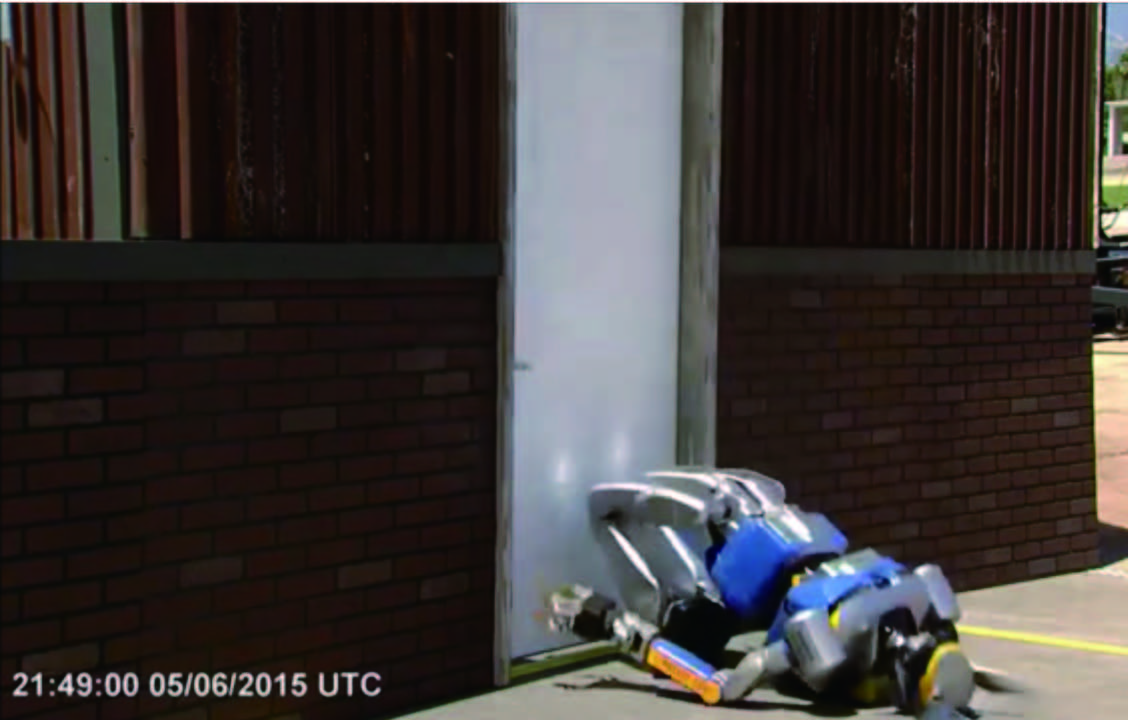
\includegraphics[width = 7.5cm]{img/drc_door_aist_day1}
  \caption{Crash accident at DRC Finals on June 5}
  \label{fig:drc_door_aist_day1}
\end{figure}

The robot failed the lever operation because the doors in DRC Finals had different latch properties
as shown in Table.\ref{tbl:door_latch}. On day1, We had hard-corded the latch rotation angle as 30 degrees,
which worked at the rehasal. Of course, such imprementation is not acceptable 
for the actual disaster responce robots.
%
\begin{table}[htb]
\caption{Door latch properties at DRC finals} \label{tbl:door_latch}
\begin{tabular}{lclc}
\hline
Course & Angle of latch release & Date & Door task result  \\ 
\hline
Green & 30 deg & June 4 (rehasal) & Success  \\
Yellow & 70 deg & June 5 (day1) & Fail \\
Blue &  50 deg & June 6 (day2)  & Success \\
\hline
\end{tabular}
\end{table}

